\documentclass[12pt]{article}

\usepackage{hyperref}
\usepackage{amsmath, mathtools}
\usepackage{amsfonts}
\usepackage{amssymb}
\usepackage{graphicx}
\usepackage{colortbl}
\usepackage{xr}
\usepackage{longtable}
\usepackage{xfrac}
\usepackage{tabularx}
\usepackage{float}
\usepackage{siunitx}
\usepackage{caption}
\usepackage{pdflscape}
\usepackage{afterpage}
\usepackage{tabu}
\usepackage{verbatim}
\usepackage{url}
\usepackage{tikz}
\usepackage{enumitem}
\usepackage{extarrows}
\usepackage{booktabs}
\usepackage[round]{natbib}
\usetikzlibrary{shapes.geometric, arrows}

\captionsetup{belowskip=12pt,aboveskip=4pt}

\makeatletter
\newcommand*\bigcdot{\mathpalette\bigcdot@{.7}}
\newcommand*\bigcdot@[2]
  {\mathbin{\vcenter{\hbox{\scalebox{#2}{$\m@th#1\bullet$}}}}}
\makeatother

%\usepackage{refcheck}

\hypersetup{
    bookmarks=true,         % show bookmarks bar?
    colorlinks=true,        % false: boxed links; true: colored links
    linkcolor=red,          % color of internal links 
                            %  (change box color with linkbordercolor)
    citecolor=blue,         % color of links to bibliography
    filecolor=magenta,      % color of file links
    urlcolor=cyan           % color of external links
}

%% Comments

\usepackage{color}

\newif\ifcomments\commentsfalse

\ifcomments
\newcommand{\authornote}[3]{\textcolor{#1}{[#3 ---#2]}}
\newcommand{\todo}[1]{\textcolor{red}{[TODO: #1]}}
\else
\newcommand{\authornote}[3]{}
\newcommand{\todo}[1]{}
\fi

\newcommand{\wss}[1]{\authornote{blue}{SS}{#1}}
\newcommand{\spc}[1]{\authornote{magenta}{SP}{#1}}
%% Common Parts

\newcommand{\progname}{MPS } % PUT YOUR PROGRAM NAME HERE



\newcommand{\sskip}{\vskip 1mm}

% For easy change of table widths
\newcommand{\colZwidth}{1.0\textwidth}
\newcommand{\colAwidth}{0.13\textwidth}
\newcommand{\colBwidth}{0.82\textwidth}
\newcommand{\colCwidth}{0.1\textwidth}
\newcommand{\colDwidth}{0.05\textwidth}
\newcommand{\colEwidth}{0.8\textwidth}
\newcommand{\colFwidth}{0.17\textwidth}
\newcommand{\colGwidth}{0.5\textwidth}
\newcommand{\colHwidth}{0.28\textwidth}

% Used so that cross-references have a meaningful prefix
\newcounter{defnum} %Definition Number
\newcommand{\dthedefnum}{GD\thedefnum}
\newcommand{\dref}[1]{GD\ref{#1}}
\newcounter{datadefnum} %Datadefinition Number
\newcommand{\ddthedatadefnum}{DD\thedatadefnum}
\newcommand{\ddref}[1]{DD\ref{#1}}
\newcounter{theorynum} %Theory Number
\newcommand{\tthetheorynum}{T\thetheorynum}
\newcommand{\tref}[1]{T\ref{#1}}
\newcounter{tablenum} %Table Number
\newcommand{\tbthetablenum}{T\thetablenum}
\newcommand{\tbref}[1]{TB\ref{#1}}
\newcounter{assumpnum} %Assumption Number
\newcommand{\atheassumpnum}{P\theassumpnum}
\newcommand{\aref}[1]{A\ref{#1}}
\newcounter{goalnum} %Goal Number
\newcommand{\gthegoalnum}{P\thegoalnum}
\newcommand{\gsref}[1]{GS\ref{#1}}
\newcounter{instnum} %Instance Number
\newcommand{\itheinstnum}{IM\theinstnum}
\newcommand{\iref}[1]{IM\ref{#1}}
\newcounter{reqnum} %Requirement Number
\newcommand{\rthereqnum}{P\thereqnum}
\newcommand{\rref}[1]{R\ref{#1}}
\newcounter{nfreqnum} %NF Requirement Number
\newcommand{\rthenfreqnum}{P\thenfreqnum}
\newcommand{\nfref}[1]{NF\ref{#1}}
\newcounter{lcnum} %Likely change number
\newcommand{\lthelcnum}{LC\thelcnum}
\newcommand{\lcref}[1]{LC\ref{#1}}
\newcommand{\sref}[1]{\S~\ref{#1}}

\usepackage{fullpage}

\begin{document}
\pagenumbering{gobble}

\title{CAS 741: SRS\\[10pt]\Large Dynamical Systems: \progname}
\author{Karol Serkis\\\texttt{serkiskj@mcmaster.ca}\\GitHub:
\href{https://www.github.com/karolserkis}{karolserkis}}
\date{\today}
	
\maketitle

~\newpage

\pagenumbering{roman}
\tableofcontents

\clearpage

\setcounter{secnumdepth}{0}

\section{Revision History}

\begin{table}[hp]
\caption{Revision History}
\begin{tabularx}{\textwidth}{llX}
\toprule
\textbf{Date} & \textbf{Developer(s)} & \textbf{Change}\\
\midrule
October 8, 2018 & Karol Serkis &  First full draft for submission\\
October 4, 2018 & Karol Serkis &  First full draft\\
October 3, 2018 & Karol Serkis & First revision and all content sections added
\\September 28, 2018 & 
Karol Serkis & First draft of document in landscape
orientation for presentation\\
September 26, 2018 & Karol Serkis & SRS presentation slides discussed with Dr.
Spencer Smith \\
December 14, 2018 & Karol Serkis & All GitHub issues and comments addressed \\
\bottomrule
\end{tabularx}
\end{table}

~\newpage

\section{Reference Material}

This section records information for easy reference: (Units, constants, 
symbols, abbreviations, and acronyms)

\subsection{Notation}

This section describes the notation conventions used in this document.

\subsubsection{Mathematical Notation}

The notation in this document follows the standard mathematical notation
conventions.
The standard mathematical spaces (specifically Euclidean space in this project)
are used for the symbols in this document (see Table of Symbols).
Example of mathematical notation usage and for double pendulum below:
$$x_1 = l_1 \sin\theta_1 \quad\quad y_1 = -l_1 \cos\theta_1$$
$$x_2 = l_1 \sin\theta_1 + l_2 \sin\theta_2 \quad\quad y_2 = -l_1\cos\theta_1
-l_2\cos\theta_2$$

\begin{figure}[h]
	\centering
	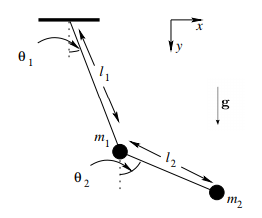
\includegraphics[width=175px]{doublepend.PNG}
\caption{A simple gravity double pendulum~\citep{SzuminskiOlsztyn2012}}
	\label{fig:doublepend}
\end{figure}

\newpage

\subsection{Table of Units}

Throughout this document SI (Syst\`{e}me International d'Unit\'{e}s) is
utilized as the unit system. In addition to the basic units, several derived
units are used as described below.  
For each unit, the symbol is given followed by a
description of the unit and the SI name.

\renewcommand{\arraystretch}{1.2}
\begin{center}
  \noindent \begin{tabular}{l l l} 
    \toprule		
    \textbf{symbol} & \textbf{unit} & \textbf{SI}\\
    \midrule 
    \si{\metre} & length & metre\\
    \si{\kilogram} & mass & kilogram\\
    \si{\second} & time & second\\
    \si{\degree} & angle & degree\\
    \bottomrule
  \end{tabular}
\end{center}

\subsection{Table of Symbols}

The table that follows summarizes the symbols used in this document along with
their units. The choice of symbols was made to be consistent with calculus, 
ordinary differentials (ODE), the Lagrangian, kinematics etc. The standard 
mathematical spaces are used (e.g. $\mathbb{N}$, $\mathbb{Z}$, $\mathbb{R}$, 
etc.) as well as some additional spaces defined in the following table. 
~\newline
\renewcommand{\arraystretch}{1.2}
\noindent \begin{longtable*}{l l l p{8cm}} \toprule
\textbf{symbol} & \textbf{space} & \textbf{unit} & \textbf{description}\\
\midrule 
$g$ & $\mathbb{R}$ & -- & gravitational constant
\\
$m_1$ & $\mathbb{R}$ & kg & mass of the 1st pendulum weight
\\ 
$m_2$ & $\mathbb{R}$ & kg & mass of the 2nd pendulum weight
\\ 
$m_n$ & $\mathbb{R}$ & kg & mass of the nth pendulum weight
\\ 
$l_1$ & $\mathbb{R}$ & m & length of the 1st pendulum rod
\\ 
$l_2$ & $\mathbb{R}$ & m & length of the 2nd pendulum rod
\\ 
$l_n$ & $\mathbb{R}$ & m & length of the nth pendulum rod
\\
$\theta_1$ & $\mathbb{R}$ & \si{\degree} & amplitude from 
the pivot point
\\
$\theta_2$ & $\mathbb{R}$ & \si{\degree} & amplitude from 
the 1st pendulum weight
\\
$\theta_n$ & $\mathbb{R}$ & \si{\degree} & amplitude from 
the nth pendulum weight
\\
$L$ & $\sum\mathbb{R}$ & -- & Pendulum system Lagrangian
\\
$T$ & $\sum\mathbb{R}$ & -- & Kinetic energy of system
\\
$V$ & $\sum\mathbb{R}$ & -- & Potential energy of system
\\
\bottomrule
\end{longtable*}
\newpage
\subsection{Abbreviations and Acronyms}

The symbols are listed in alphabetical order.\\

\renewcommand{\arraystretch}{1.2}
\begin{tabular}{l l} 
  \toprule		
  \textbf{symbol} & \textbf{description}\\
  \midrule 
  A & Assumption\\
  DD & Data Definition\\
  GD & General Definition\\
  GS & Goal Statement\\
  IM & Instance Model\\
  LC & Likely Change\\
  NF & Non-Functional Requirement\\
  PS & Physical System Description\\
  R & Requirement\\
  SRS & Software Requirements Specification\\
  T & Theoretical Model\\
  \bottomrule
\end{tabular}

\newpage

\pagenumbering{arabic}

\setcounter{secnumdepth}{3}

\section{Introduction}

This documents is an SRS for the \progname program. The
directory for this project can be found at GitHub:
\href{https://github.com/karolserkis/CAS-741-Pendula/}
{/karolserkis/CAS-741-Pendula/}\\
This SRS template is based on~\citep{SmithAndLai2005} \&~\citep{SmithEtAl2007}
(ex. based on the principle of information hiding~\citep{Parnas1972a}).

\subsection{Purpose of Document}
The purpose of this document is to describe the requirements for finding a 
solution for a Multi-Pendulum Simulation ( \progname) program and tracking the 
chaotic motion of the system. 

The theoretical models used in the \progname code will be provided, insuring
assumptions and unambiguous definitions are identified. This document 
is intended to be used as a reference to provide all information necessary to 
understand and verify the inputs to outputs. The SRS is abstract: the contents 
describe the problem being solved, but not how to solve it.

This document will be used as a starting point for subsequent development
phases, including writing the design specification and the software 
verification and validation plan. The verification and validation plan 
will show the steps in the software documentation/implementation.

\subsection{Scope of Requirements} 

The scope of the \progname program is limited to the generation 
of a plot trajectory simulation and other related plots.
This document is to describe the requirements for a
\progname program solution that only focuses on multi-pendulum simulations 
and tracking the chaotic motion of the system. 
It will allow users to generate plot trajectories over time using ODE/DAE 
initial value problem solvers. In the case of a double pendulum you have 
a new system that is dynamic and chaotic and
requires a set of coupled ordinary differential equation solvers. Once one
introduces multiple pendulums the system becomes chaotic 
and interesting to model and simulate. 

Assumptions: The \progname will be a closed system. 
Air resistance and friction will not be considered for the simulation. 
The \progname will be limited to the user initialized inputs and
the output of the \progname will either plot trajectories over time and 
limit the user to a specific duration of the simulation, 
in order to allow diagrams and trajectory history to be saved. 
The plot trajectory simulation should run on a local system 
(personal computer) that is capable of executing the simulation without serious 
performance problems.
The user will be able to set a range of time and initialize the system. \\

\subsection{Characteristics of Intended Reader} 
Simplification of some physical concepts are proposed to make the document
technically accessible and also the software to be accessible.
Nevertheless, the intended reader is expected to have a basic knowledge in
mathematics (calculus, differentials/ODEs) and physics (kinematics, kinetic 
energy, potential energy, Lagrangian) to get a deeper understanding of 
the document.

\subsection{Organization of Document}
\begin{itemize}
\item This document follows the template outlined in \citet{SmithAndLai2005} 
\item The presentation follows the standard pattern of presenting goals,
theories, definitions, and assumptions.
\item The goal statements are refined to the theoretical models, and the
theoretical
models to the instance models. The data definitions are used to support the
definitions of the different models.
\end{itemize}

\section{General System Description}
This section identifies the interfaces between the system and its environment,
describes the user characteristics and lists the system constraints.

\subsection{System Context}

\begin{center}
\framebox{\textbf {USER}} $ \xLongrightarrow[\textbf{ex. num of pendula, 
toggle plot}]{\textbf{User Input}} $\framebox{\textbf { \progname}}
$ \xLongrightarrow[\textbf{ex. GUI, trajectory simulation, plots}] 
{\textbf{Output to the Usere}}$\framebox{\textbf {USER}}\\
\end{center}

\begin{itemize}
\item User Responsibilities:
\begin{itemize}
\item Ensure that the input data is fits the system model (i.e. correct value,
only positive integers, when required) 
(For example, weights and lengths and other appropriate units found in 
Table of Units and Symbols)
\item Ensure that the input data is of the correct type 
(i.e. Enter an integer not char or string when integer is asked for)
\end{itemize}
\item \progname program Responsibilities:
\begin{itemize}
\item Detect data type mismatch, such as a string of characters instead of a
  floating point number.
\item Determine if the inputs satisfy the required physical and software 
  constraints.
\item Solve the system of equations arising from the input data to generate 
  the output data.
\item Generate a plot of the output data and generate diagrams 
to display to the user.
\item Ensure that simulation is within the scope of the simulation window 
(For example the number of pendulums cannot exceed the boundry of the
GUI window of the simulation)
\end{itemize}
\end{itemize}

\subsection{User Characteristics}
The end user of \progname program should have an understanding of first year 
undergraduate math and physics. Less understanding of physics and math are
required to use the software than understand
this document or the inner workings of the software program.

\subsection{System Constraints}
The system constraint will be the display requirements for the GUI and thus 
a contraint on the number of pendula possible to be displayed 
in the simulation.

\newpage
\section{Specific System Description}

This section first presents the problem description, which gives a high-level
view of the problems to be solved and the motivation behind \progname software.
This is followed by the solution
characteristics specification, which presents the assumptions, theories, 
definitions and finally the instance models.

\subsection{Problem Description}

The \progname software will generate a plot trajectory in a 3D plot grid.
A simple gravity pendulum is very easy to system to model and consists of a
weight suspended from a pivot and the weight is given enough space to swing
freely. To simplify the model we assume no air resistance with a friction-less
pivot. The model and calculations for the simple gravity pendulum are well
defined and only require simple derivations and differential solvers.

\progname program will produce a simulation given a set of constants and input 
(starting position away from equilibrium position).
Terminologies and the physical system are described below.

\subsubsection{Terminology and Definitions}

This subsection provides a list of terms that are used in the subsequent
sections and their meaning, with the purpose of reducing ambiguity and making
it easier to correctly understand the requirements:

\begin{description}
\item[Equilibrium position:] The pendulum rod and weight position in its 
resting state.
\item[3D Cartesian coordinate system:] The pendulum rod and weight swing from a
pivot position origin $(x,y,z)$
\end{description}

\begin{figure}[H]
	\centering
	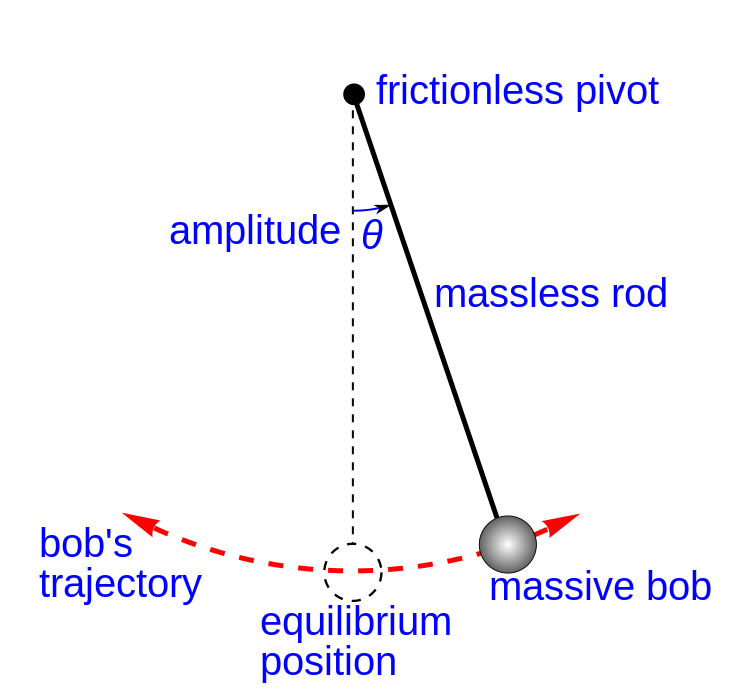
\includegraphics[width=180px]{simple-pend.png}
\caption{A simple gravity pendulum where the model assumes no friction or air
resistance}
	\label{fig:maxresdefault}
\end{figure}

\begin{description}
\item[Lagrangian:] The Lagrangian equation $L=T-V$, where $T$ and $V$ are 
the kinetic and potential energies of the system respectively.
\item[Poincaré map:] Starting with the Poincaré section of the \progname 
in 3D space, the Poincaré map $P$ is a projection from point $x$ onto point 
$P(x)$ transforming the 3D space into a 2D projection diagram plot.
\end{description}

\subsubsection{Physical System Description}

The physical system of \progname program includes the following elements:

\begin{itemize}
\item[PS1:] Simulate an n-rod multi-pendulum system with no friction and no air
resistance in a 3D space.
\end{itemize}

\begin{figure}[H]
	\centering
	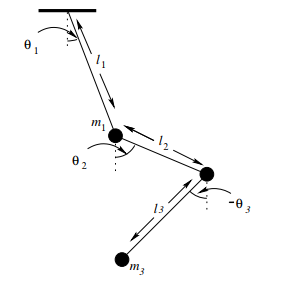
\includegraphics[width=190px]{triplependula.PNG}
\caption{A triple pendulum example~\citep{SzuminskiOlsztyn2012}.
See Table of Symbols for more info.}
	\label{fig:maxresdefault}
\end{figure}

\subsubsection{Goal Statements}

\noindent Given the user input and the initial state of the \progname with 
reference to the table of symbols the goal statements are: 

\wss{Isn't the initial state of the multi-pendulum part of the input?}

\begin{itemize}
\item[GS\refstepcounter{goalnum}\thegoalnum:] Generate a trajectory plot of 
the movement of the pendula from user input starting state to equilibrium 
state of rest and show logged statistics over time to the user. 
\wss{I believe you are assuming no friction,
so I don't think the pendula will come to a state of rest.}
\item[GS\refstepcounter{goalnum}\thegoalnum:] Generate a Poincaré map plot of 
the movement of the pendula from user input starting state to equilibrium 
state of rest.
\end{itemize}

\wss{Your goals are focused on plots.  A more abstract output would be to
  generate the trajectory, without the word plot. You can still make generating
  a plot part of the requirements, but it would also be nice to see the option
  of outputting the results to a file}

\newpage

\subsection{Solution Characteristics Specification}

\subsubsection{Assumptions}

This section simplifies the original problem and helps in developing the
theoretical model by filling in the missing information for the physical
system. The numbers given in the square brackets refer to the theoretical model
[T], general definition [GD], data definition [DD], instance model [IM], or
likely change [LC], in which the respective assumption is used.

\begin{itemize}
\item[A\refstepcounter{assumpnum}\theassumpnum \label{A:equation}:]
In the model we assume no air resistance with a friction-less pivot, moving in
space with respect to the Lagrangian calculations made. [T1][DD1][IM1] 
\wss{You need to explicitly invoke these assumptions when they apply, 
not just list them.}
\item[A\refstepcounter{assumpnum}\theassumpnum \label{A:kinetic}:]
  The kinetic energy will be represented by real-value and will fit the 
mathematical model and scope. [T2][DD1]
\item[A\refstepcounter{assumpnum}\theassumpnum \label{A:poten}:]
  The potential energy will be represented by real-value and will fit the 
mathematical model and scope. [T3][DD1]
\item[A\refstepcounter{assumpnum}\theassumpnum \label{A:init-user}:]
The user knows what the purpose of the simulation model and inputs weights and 
lengths according to possible simulation characteristics. 
[DD1][IM1][T1][T2][T3][T4]
\end{itemize}

\wss{Don't you need the assumption that the angles are small enough that sin
  theta equals theta?}

\wss{I believe you should have an assumptions that the connecting rods are
  mass-less.}

\newpage

\subsubsection{Theoretical Models}\label{sec_theoretical}

This section focuses on the general equations and laws that \progname program 
is based on.\\

\noindent
\begin{minipage}{\textwidth}
\renewcommand*{\arraystretch}{1.5}
\tabulinesep=1.5mm
\begin{tabu}{| p{\colAwidth} | p{\colBwidth}|}
  \hline
  \rowcolor[gray]{0.9}
  Number& T\refstepcounter{theorynum}\thetheorynum \label{lagrangian}\\
  \hline
  Label&\bf Double Pendulum Lagrangian ($L=T-V$)\\
  \hline
  Equation&  
$$L =\frac{1}{2}(m_1 + m_2) l_1^2 \dot{\theta}_1^2 + \frac{1}{2}m_2 l_2^2
\dot{\theta}_2^2 + m_2l_1l_2\dot{\theta}_1\dot{\theta}_2 \cos(\theta_1 -
\theta_2)$$
    $$+ (m_1 + m_2) g l_1 \cos\theta_1 + m_2 g l_2\cos\theta_2$$\\
  \hline
  Description & Lagrangian model system solution\\
  \hline
  Source & ~\citep{DiegoAssencioLagrang}\\
  \hline
  Ref.\ By & [A1][A4] \wss{Use cross-references to generate these, 
rather than hard-coding.}\\
  \hline
\end{tabu}
\end{minipage}

\wss{How is this equation derived?}
\wss{I would think you would have theoretical models on kinetic energy and
  potential energy, defined in an abstract way, so that they would be useful 
  for other problems.}
\wss{These models are for a double pendulum, but the problem is supposed to 
  have more than two pendulums.}

\noindent
\begin{minipage}{\textwidth}
\renewcommand*{\arraystretch}{1.5}
\tabulinesep=1.5mm
\begin{tabu}{| p{\colAwidth} | p{\colBwidth}|}
  \hline
  \rowcolor[gray]{0.9}
  Number& T\refstepcounter{theorynum}\thetheorynum \label{kinetic}\\
  \hline
  Label&\bf Double Pendulum Kinetic Energy\\
  \hline
  Equation&  
$$ T = \displaystyle\frac{1}{2}m_1v_1^2 + \frac{1}{2}m_2v_2^2 $$
$$ = \frac{1}{2}m_1(\dot{x}_1^2 + \dot{y}_1^2) + \frac{1}{2}m_2(\dot{x}_2^2 +
\dot{y}_2^2) $$
$$ = \frac{1}{2}m_1 l_1^2 \dot{\theta}_1^2 + \frac{1}{2}m_2\left[l_1^2
\dot{\theta}_1^2 + l_2^2 \dot{\theta}_2^2 + 2l_1l_2\dot{\theta}_1\dot{\theta}_2
\cos(\theta_1 - \theta_2)\right]$$\\
  \hline
  Description & Potential Energy model system solution\\
  \hline
  Source & ~\citep{DiegoAssencioLagrang}\\
  \hline
  Ref.\ By & [A2][A4]\\
  \hline
\end{tabu}
\end{minipage}

\noindent
\begin{minipage}{\textwidth}
\renewcommand*{\arraystretch}{1.5}
\tabulinesep=1.5mm
\begin{tabu}{| p{\colAwidth} | p{\colBwidth}|}
  \hline
  \rowcolor[gray]{0.9}
  Number& T\refstepcounter{theorynum}\thetheorynum \label{potential}\\
  \hline
  Label&\bf Double Pendulum Potential Energy\\
  \hline
  Equation&  
$$V = m_1 g y_1 + m_2gy_2$$
$$= -m_1 g l_1 \cos\theta_1 - m_2 g (l_1 \cos\theta_1 + l_2 \cos\theta_2)$$
$$= -(m_1 + m_2) g l_1 \cos\theta_1 - m_2 g l_2\cos\theta_2$$\\
  \hline
  Description & Potential Energy model system solution\\
  \hline
  Source & ~\citep{DiegoAssencioLagrang}\\
  \hline
  Ref.\ By & [A3][A4]\\
  \hline
\end{tabu}
\end{minipage}\\

\subsubsection{General Definitions}\label{sec_gendef}

We will use the Lagrangian and ODEs. No need for general definitions in
current documentation.

\subsubsection{Data Definitions}\label{sec_datadef}

This section collects and defines all the data needed to build the instance
models. The models here are to satisfy the theoretical models constrained and 
closed 3D space.\\

\noindent
\begin{minipage}{\textwidth}
\renewcommand*{\arraystretch}{1.5}
\tabulinesep=1.5mm
\begin{tabu}{| p{\colAwidth} | p{\colBwidth}|}
  \hline
  \rowcolor[gray]{0.9}
  Number& DD\refstepcounter{datadefnum}\thedatadefnum \label{real-interv}\\
  \hline
  Label&\bf Closed, Real intervals\\
  \hline
  Equation&  
$$\mathbb{R} (\texttt{for Langrangian equation})$$
$$ P(x) :\mathbb{Z} \times \mathbb{R} \implies \mathbb{R}$$\\
  \hline
  Description & Simple cartesian coordinate model system solution\\
  \hline
  Source & ~\citep{DiegoAssencioLagrang}\\
  \hline
  Ref.\ By & T1,T2,T3,T4,T5\\
  \hline
\end{tabu}
\end{minipage}

\wss{I don't know what this means/}

\subsubsection{Instance Models} \label{sec_instance}    

This section transforms the problem defined in problem description into 
one which is expressed in mathematical terms. \\

\noindent
\begin{minipage}{\textwidth}
\renewcommand*{\arraystretch}{1.5}
\tabulinesep=1.5mm
\begin{tabu}{| p{\colAwidth} | p{\colBwidth}|}
  \hline
  \rowcolor[gray]{0.9}
  Number& IM\refstepcounter{instnum}\theinstnum \label{add-real}\\
  \hline
  Label&\bf Addition of closed, real intervals\\
  \hline
  Equation&  
$$\sum \mathbb{R} (\texttt{for Langrangian equation})$$
$$ P(x) :\mathbb{Z} \times \mathbb{R} \implies \mathbb{R}$$\\
  \hline
  Description & Simple cartesian coordinate model system solution\\
  \hline
  Source & ~\citep{DiegoAssencioLagrang}\\
  \hline
  Ref.\ By & T1,T2,T3,T4,T5\\
  \hline
\end{tabu}
\end{minipage}

\wss{The instance model is the most refined version of your problem that is
  closest to the eventual code. I don't understand how the above IM fits in to
  this. If anything, isn't this a data definition? Why is it even necessary?
  Are you using interval arithmetic? I would think the ODEs that you are going
  to solve are your IMs. Your theoretical models look more like IMs. Your
  theoretical models could then be replaced with more abstract versions of the
  general concepts of Lagrangian etc. The theoretical models are supposed to be
  something that could be reused in a different project.}

\subsubsection{Data Constraints} \label{sec_DataConstraints}    

The data constraints on the input and output variables, respectively.  
The column for physical constraints gives the physical limitations on 
the range of values that can be taken by the
variable. The column for software constraints restricts the range of inputs to
reasonable values.  The constraints are conservative, to give the user of the
model the flexibility to experiment with unusual situations.  The column of
typical values is intended to provide a feel for a common scenario.  The
uncertainty column provides an estimate of the confidence with which the
physical quantities can be measured.  This information would be part of the
input if one were performing an uncertainty quantification exercise.

\begin{itemize}
\item Constraint on gravity: g = $9.8 m/s^2$
\end{itemize}

\wss{What about the constraint that your lengths have to be positive? Are there
  any bounds on the initial angles? Aren't they supposed to be small? What
  about your masses?}

\subsubsection{Properties of a Correct Solution}

\noindent
A correct solution must satisfy the system of non-linear equations described. 
The user will also be able to judge the results based on the knowledge about 
the model and input.

\wss{The properties here should be something in addition to meeting the
  requirements. Meeting the requirements is a given. We are interested here in
  identifying things that should be true, but that are independent of the
  requirements. In your case, a correct solution should conserve energy. The
  energy at the start should be maintained as the simulation proceeds.}

\newpage
\section{Requirements}

This section provides the functional requirements, the business tasks that the
software is expected to complete, and the nonfunctional requirements, the
qualities that the software is expected to exhibit.


\subsection{Functional Requirements}

\noindent \begin{itemize}

\item[R\refstepcounter{reqnum}\thereqnum \label{funinput}:] \progname 
program should be able to have axis labels \& 3D Cartesian coordinates. 

\item[R\refstepcounter{reqnum}\thereqnum \label{funinput}:] \progname program 
  will take the following inputs: \wss{It would be nice to use symbols to 
  represent the inputs. You also want a way to identify how 
  many masses you have.}
  \begin{enumerate} \item The initial mass of the weights. 
      \wss{This is a confusing sentence, since mass and weight are different 
      concepts. If you use a symbol, like $m_i$ then you could probably 
      simplify the presentation.}
                    \item The initial length of the rods.
  \end{enumerate}
                    
\item[R\refstepcounter{reqnum}\thereqnum \label{funkinpot}:] \progname program 
will calculate the kinetic and potential energy after the user has set the 
initialization parameters of input from the user have been entered.

\item[R\refstepcounter{reqnum}\thereqnum \label{funlagham}:] \progname program 
will calculate the Lagrangian (and Hamiltonian (differential on Lagrangian) 
if needed) after the user has set the initialization parameters of input 
have been entered and the kinetic and potential energy of the system as whole 
has been calculated. \wss{This is
  the only time you mention the Hamiltonian. You should define it in your
  documentation, or not mention it.}

\item[R\refstepcounter{reqnum}\thereqnum \label{funplot}:] \progname program
will ensure that the inputs do not violate the constraints specified in the 
Data Constraints section:
    \begin{enumerate} \item \progname program will 
generate diagrams with and plot lines and timeline of logged movement. 
\item The timeline of swings of the pendulum will be logged and eventually
return to a resting state in equilibrium
\end{enumerate}

\end{itemize}
\newpage
\subsection{Nonfunctional Requirements}

\progname program will be try to be small and simple, so performance is not a 
priority. Any reasonable implementation will be very quick and use minimal 
storage. Rather than performance, the non-functional requirement priorities 
are correctness, understand-ability, re-usability, maintainability, and 
portability. 

\begin{itemize}
\item[NF\refstepcounter{nfreqnum}\thenfreqnum:] \progname program should be 
reliable and portable and easy to use for beginners or experts.
\end{itemize}

\subsubsection*{Correctness}
\begin{itemize}
\item The \progname tool must be correct in its generation 
of plot trajectories.
\end{itemize}

\subsubsection*{Reliability}

The \progname should run successfully and have error checking for user input.

\subsubsection*{Robustness}
\begin{itemize}
	\item The \progname must be able to recognize violated data 
	constraints and report them to the user.
	\item The \progname tool must inform the user when it encounters any 
	unspecified state.
\end{itemize}

\subsubsection*{Performance}
Performance is a priority in the \progname specification. 
It needs to be able to generate a plot reasonable amount of time.

\subsubsection*{Verify-ability}
\begin{itemize}
	\item The \progname must be verifiable with respect to the 
	correctness of its calculations. The calculation 
	procedures used by the \progname tool must be implemented such that 
	they can be verified using mathematical proofs.
\end{itemize}

\subsubsection*{Usability}
\begin{itemize}
\item The user must be able to enter values using standard mathematical 
notation.
\item The plot should generate and be large enough for 
the user's display.
\end{itemize}

\subsubsection*{Maintainability}
\begin{itemize}
	\item The evolve-ability of the \progname must allow the addition 
	of real intervals.
\end{itemize}

\subsubsection*{Re-usability}
Reusability is not a priority because there are currently no future products 
that will rely on \progname

\subsubsection*{Portability}
To ensure the portability, the \progname software will be multi-platform.

\wss{Your NFRs are ambiguous. You might have been better off with the blanket
  statement in the first paragraph, since the list of qualities brings 
  attention to the fact that what you have stated is not measurable.}

\newpage

\section{Likely Changes}    

\noindent \begin{itemize}

\item[LC\refstepcounter{lcnum}\thelcnum \label{only2dsim}:] Generation of 
simulation only in 2D
\item[LC\refstepcounter{lcnum}\thelcnum \label{only2dplot}:] Generation of 
plot and diagrams only in 2D
\item[LC\refstepcounter{lcnum}\thelcnum \label{maybe-mpi}:] Generation of 
diagrams using distributed/parallel computing

\end{itemize}

\section{Traceability Matrices and Graphs}

The purpose of the traceability matrices is to provide easy references on what
has to be additionally modified if a certain component is changed. Every time a
component is changed, the items in the column of that component that are marked
with an ``X'' may have to be modified as well. 

% Table~\ref{Table:trace} shows the
%dependencies of theoretical models, general definitions, data definitions, and
%instance models with each other. Table~\ref{Table:R_trace} shows the
%dependencies of instance models, requirements, and data constraints on each
%other. Table~\ref{Table:A_trace} shows the dependencies of theoretical models,
%general definitions, data definitions, instance models, and likely changes on
%the assumptions.

%\afterpage{
%\begin{landscape}
\begin{table}[h!]
\centering
\label{Table:A_trace}
\begin{tabular}{|c|c|c|c|c|}
\hline
	& \aref{A:equation} 
	& \aref{A:kinetic}
	& \aref{A:poten}
	& \aref{A:init-user} \\
\hline
\tref{lagrangian} & X &  &  & X \\ \hline
\tref{kinetic} &  & X &  & X \\ \hline
\tref{potential} &  &  & X & X \\ \hline
\tref{poincare} &  &  &  & X \\ \hline
\ddref{real-interv} & X & X & X & X \\ \hline
\iref{add-real} & X & X & X & X \\ \hline
\lcref{only2dsim} & X & X & X & X \\ \hline
\lcref{only2dplot} & X & X & X & X \\ \hline
\lcref{maybe-mpi} & X & X & X & X\\ \hline
\end{tabular}
\caption{Traceability Matrix Showing the Connections Between Assumptions 
and Other Items}

\end{table}
%\end{landscape}
%}

\begin{table}[h]
	\centering
	\label{Table:trace}
	\begin{tabular}{|c|c|c|c|c|c|c|}
		\hline        
		& \tref{lagrangian}
		& \tref{kinetic}
		& \tref{potential}
		& \tref{poincare}
		& \ddref{real-interv}
		& \iref{add-real} \\
		\hline
        \tref{lagrangian} & X & X & X & X & X & X \\ \hline
        \tref{kinetic} & X & X & X & X & X & X\\ \hline
        \tref{potential} & X & X & X & X & X & X\\ \hline
        \tref{poincare} &  &  &  &  & X & X\\ \hline
        \ddref{real-interv} & X & X & X &  & X & X\\ \hline
        \iref{add-real} & X & X & X &  & X & X\\ \hline
	\end{tabular}
	\caption{Traceability Matrix Showing the Connections Between Items of 
	Different Sections}
\end{table}


\begin{table}[h!]
	\centering
	\begin{tabular}{|c|c|c|c|c|c|c|}
		\hline        
		& \tref{lagrangian}
		& \tref{kinetic}
		& \tref{potential}
		& \tref{poincare}
		& \ddref{real-interv}
		& \iref{add-real} \\
		\hline
        \rref{funinput} & X & X & X &  & X & X \\ \hline
        \rref{funkinpot} & X & X & X & X & X & X\\ \hline
        \rref{funlagham} & X & X & X &  & X & X \\ \hline
        \rref{funplot} & X & X & X & X & X & X\\ \hline
	\end{tabular}
	\caption{Traceability Matrix Showing the Connections Between 
	Requirements and Instance Models}
	\label{Table:R_trace}
\end{table}

%The purpose of the traceability graphs is also to provide easy references on
%what has to be additionally modified if a certain component is changed.  The
%arrows in the graphs represent dependencies. The component at the tail of an
%arrow is depended on by the component at the head of that arrow. Therefore, if 
%a
%component is changed, the components that it points to should also be
%changed. Figure~\ref{Fig_ATrace} shows the dependencies of theoretical models,
%general definitions, data definitions, instance models, likely changes, and
%assumptions on each other. Figure~\ref{Fig_RTrace} shows the dependencies of
%instance models, requirements, and data constraints on each other.

% \begin{figure}[h!]
% 	\begin{center}
% 		%\rotatebox{-90}
% 		{
% 			\includegraphics[width=\textwidth]{ATrace.png}
% 		}
% 		\caption{\label{Fig_ATrace} Traceability Matrix Showing the 
%		Connections Between Items of Different Sections}
% 	\end{center}
% \end{figure}

% \begin{figure}[h!]
% 	\begin{center}
% 		%\rotatebox{-90}
% 		{
% 			\includegraphics[width=0.7\textwidth]{RTrace.png}
% 		}
% 		\caption{\label{Fig_RTrace} Traceability Matrix Showing the 
%		Connections Between Requirements, Instance Models, 
%		and Data Constraints}
% 	\end{center}
% \end{figure}

\newpage

\bibliographystyle {plainnat}
\bibliography {../../ReferenceMaterial/References}

\end{document}
